\subsection{DIP}
\label{sec:algorithms:dip}

\begin{figure}
    \centering
    \begin{subfigure}[b]{0.50\textwidth}
        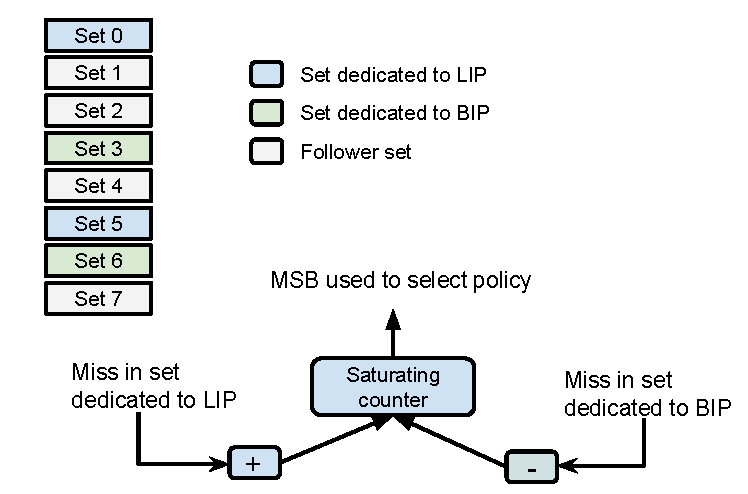
\includegraphics[width=\textwidth]{figures/algorithms/DIP_architecture}
        \caption{Set-dueling architecture.}
        \label{fig:algorithms:dip:set_dueling}
    \end{subfigure}    
    \begin{subfigure}[b]{0.45\textwidth}
        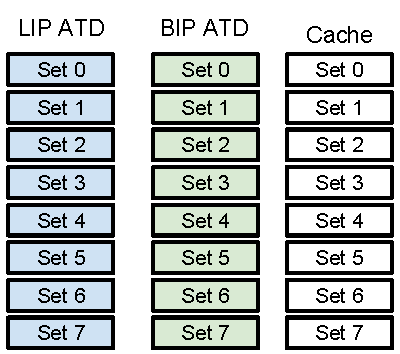
\includegraphics[width=.9\textwidth]{figures/algorithms/DIP_atd_architecture}
        \caption{ATD architecture.}
        \label{fig:algorithms:dip:atd}
    \end{subfigure}
    \caption{Alternate \gls{dip} organizations.}
\end{figure}

\gls{dip}~\cite{Qureshi2007} was originally proposed in 2007.
The \gls{dip} algorithm views the cache set as a stack, as in \gls{lru}.
Replacement and promotion policies are equal to \gls{lru}, \gls{dip} evicts the block at the \gls{lru} position, and following a cache hit a block moves to the \gls{mru} position.
In contrast to \gls{lru}, \gls{dip} is a combination of two insertion policies, the standard \gls{lip} and \gls{bip}.
\gls{lip} inserts new blocks at the \gls{mru} position.
\gls{bip} inserts new blocks either at the \gls{lru} position or with a small probability, $p = \frac{1}{32}$, at the \gls{mru} position. 
The overall \gls{dip} algorithm switches between the two insertion policies by always using the one that is expected to cause fewer cache misses.

By mostly inserting at the \gls{lru} position the \gls{bip} insertion policy can theoretically handle trashing memory access patterns.
When most new blocks enter at the \gls{lru} position, the upper parts of the \gls{lru} stack can contain blocks that have been re-referenced.
In a trashing access pattern, this results in part of the working set residing in the upper part of the stack while the rest are inserted at the \gls{lru} position and evicted at the next miss.
By sometimes inserting at the \gls{mru} position \gls{bip} will give blocks not referenced by the next miss a chance to stay in the cache. 
Inserting at the \gls{mru} position will also force stale cache blocks in the upper part of the stack to move towards the \gls{lru} position.

The authors of \gls{dip} present several methods to detect the best of the two replacement algorithms, one of them is set-dueling.
Set-dueling is implemented by having some sets of the cache always use \gls{bip} and some always use \gls{lip}.
A counter tracks the performance of the dueling sets.
Misses in \gls{lip} sets will increment the counter and misses in \gls{bip} sets will decrement the counter.
The \gls{msb} of the counter can then be used to select the best performing of the two algorithms.
If the \gls{msb} is one, an overweight of misses in \gls{lip} sets are occurring, and \gls{bip} is the best performing algorithm. 
If the \gls{msb} is zero, then an overweight of \gls{bip} misses are occurring, and \gls{lip} is the best performing algorithm.
Figure~\ref{fig:algorithms:dip:set_dueling} shows the set dueling and algorithm selection architecture.
In the figure sets 0 and 5 are dueling sets for \gls{lip} while 3 and 6 are dueling sets for \gls{bip}.
All other sets are follower sets, meaning that they utilize the algorithm indicated by the selection logic.

Another solution is to utilize two \glspl{atd}, as shown in Figure~\ref{fig:algorithms:dip:atd}.
An \gls{atd} is equal to the cache's tag directory; it keeps track of blocks present but does not store any data.
\glspl{atd} are, for this reason, cheaper than a full cache, but still requires more storage than duel-sets that use the existing cache.
As the figure shows, the two \glspl{atd} run one algorithm each and all operations on the main cache execute in parallel on the \glspl{atd}.
The same counter architecture controlled by misses in either \gls{atd} is used to select the best performing algorithm for the main cache.
The main advantage of using an \gls{atd} is that all available information is used when selecting between \gls{bip} and \gls{lip}.
Also, the entire cache will always use the best algorithm while in set-dueling a fraction of the sets will always run the worst performing algorithm.
The difference between using an \gls{atd} and cache dueling sets in terms of misses were shown to be small in the original paper.
On their benchmarks, they measured an average decrease in misses by 22.3\% using \glspl{atd}, compared to a 21.3\% decrease when using 32 duel-sets~\cite{Qureshi2007}, on a 4096 set cache.

Figure~\ref{fig:algorithms:bip_example} shows an example cache set managed by \gls{dip}.
In the example, we assume \gls{bip} insertion with no insertions at the \gls{mru} position.
In the initial state, there are four blocks; A, B, C, and D.
A is at the \gls{mru} position and D is at the \gls{lru} position.
The first request is for C; this is a hit, and C is promoted to the \gls{mru} position, A and B are pushed towards the \gls{lru} position.
Then follows a request for E, which is a miss.
\gls{dip} evicts D at the \gls{lru} position, and E is inserted in its place.
Then follows two requests to D; the first request is a miss causing E to be evicted and D to be inserted at the \gls{lru} position.
The second request is a hit and promotes D to \gls{mru}, pushing all other blocks one step towards the \gls{lru} position.

\begin{figure}[th]
    \centering
    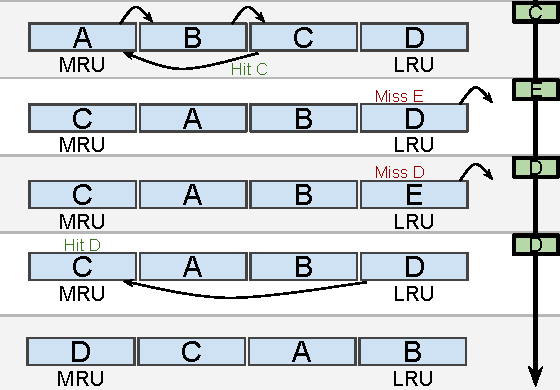
\includegraphics[width=.65\textwidth]{figures/algorithms/DIP}
    \caption[DIP managed 4-way cache set.]{\gls{dip} managed 4-way cache set. (Assuming \gls{bip} insertion)}
    \label{fig:algorithms:bip_example}
\end{figure}
